\documentclass{homework}
\usepackage{listings}
\usepackage{courier}
\usepackage{booktabs}
\usepackage{siunitx}  % Pretty scientific notation

\newcommand{\hwclass}{Math 6601}
\newcommand{\hwname}{Jacob Hauck}
\newcommand{\hwtype}{Homework}

\newcommand{\mat}[1]{\left[\begin{matrix}#1\end{matrix}\right]}
\newcommand{\R}{\textbf{R}}
\newcommand{\bigoh}{\mathcal{O}}
\newcommand{\dee}{\;\text{d}}
\DeclareMathOperator{\cond}{cond}
\DeclareMathOperator{\spn}{span}
\DeclareMathOperator{\sgn}{sgn}

\newcommand{\hwnum}{6}
\renewcommand{\questiontype}{Problem}

\begin{document}
	\maketitle
	
	\question Set $x_i = i-3$ for $i=1,2,\dots, 6$. If $q(x) = p(x) + r(x)$, then $q(x)$ will take the required values on $\{x_i\}_{i=1}^6$ provided that $r(x_6) = 31$ and $r(x_i) = 0$ if $1\le i <6$. We can ensure that $r(x)$ is a polynomial passing through these points by using polynomial interpolation. In the Lagrange form, this means that
	\begin{equation*}
		r(x) = \sum_{k=1}^n r(x_k)L_k(x)= r(x_6)L_6(x) = 31\prod_{i=1}^5\frac{x-x_i}{x_6 - x_i} = 31\cdot\frac{x+2}{5}\cdot\frac{x+1}{4}\cdot\frac{x}{3}\cdot\frac{x-1}{2}\cdot(x-2).
	\end{equation*}
	Then
	\begin{equation*}
		q(x) = p(x) + r(x) = x^4 - x^3 + x^2 -x+ 1 - \frac{31}{120}(x+2)(x+1)x(x-1)(x-2)
	\end{equation*}
	is a polynomial that takes the required values.
	
	\question Since $P_3$ has degree less than or equal to 3, we can write $P_3(x) = 6x^3 + bx^2 + cx + d$ for some constants $a,b,c,d$. Then $P_3(0) = 0$ implies that $d = 0$, and the remaining interpolation points yield the system of equations
	\begin{align*}
		8y &= 6 + 2b + 4c \\
		3 &= 6 + b + c \\
		2 &= 48 + 4b + 2c.
	\end{align*}
	Solving the last two equations by elimination gives $-4 = 36 + 2b \implies b = -20$, and $c = -3 -b = 17$. Thus, $8y =  6 -40 + 68 = 34$, so $y = \frac{17}{4}$.
	
	\question Since $S(x)$ is a cubic spline, it must satisfy $S_0(2) = S_1(2)$, and $S_0'(2) = S_1'(2)$, and $S_0''(2) = S_1''(2)$. Then
	\begin{equation*}
		a = S_1(2) = S_0(2) = 3 + 2 - 1 = 4,
	\end{equation*}
	and
	\begin{equation*}
		b = S_1'(2) = S_0'(2) = 3 + 4 - 3 = 4,
	\end{equation*}
	and
	\begin{equation*}
		2c = S_1''(2) = S_0''(2) = 4 - 6 = -2.
	\end{equation*}
	Thus, $a= 4$, $b=4$, and $c= -1$.
	
	\question Let $A$ be strictly diagonally dominant. Then $Ax = b$ has a unique solution.
	\begin{proof}
		Let $R_i$ be the Gershgorin radius for the $i$th row of $A$, that is,
		\begin{equation*}
			R_i = \sum_{j\ne i} |a_{ij}|,
		\end{equation*}
		where $A=\{a_{ij}\}$. Then, by the assumption of strict diagonal dominance, it follows that $|a_{ii}| > R_i$ for all $i$. Hence, for any $i$, we have $|0 - a_{ii}| = |a_{ii}| > R_i$, which implies that $0 \notin \{z \in \mathbb{C} : |z - a_{ii}| < R_i\} = D_i$, the Gershgorin disc for the $i$th row of $A$. Thus, $0$ does not belong to any of the Gershgorin discs of $A$, so $0$ cannot be an eigenvalue of $A$ by the Gershgorin circle theorem. This implies that all the eigenvalues $\lambda_1, \dots, \lambda_n$ of $A$ are nonzero. Then
		\begin{equation*}
			\det(A) = \prod_{i=1}^n \lambda_i \ne 0,
		\end{equation*}
		which implies that $Ax = b$ has a unique solution.
	\end{proof}
	
	\question 
	\begin{alphaparts}
		\questionpart Using the notation from the slides, we must have $a_0 = 0$, and $a_1 = 4$. The condition $S_0''(1) = 4$ forces us to take $c_0 = 2$, as $2c_0 = S_0''(1)$. From the conditions $S_1(2) = S_0(2)$, $S_1'(2) = S_0'(2)$ and $S_1''(2) = S_0''(2)$, we get
		\begin{align*}
			4 = a_1 &= a_0 + b_0 + c_0 + d_0 = 2 +b_0  +d_0\\
			b_1 &= b_0 + 2c_0 + 3d_0 = 4 + b_0 + 3d_0\\
			2c_1 &= 2c_0 + 6d_0 = 4 + 6d_0,
		\end{align*}
		and from the conditions $S_1(3) = 8$ and $S_1''(3) = 4$ as well as the above equations, we get
		\begin{align*}
			8 &= a_1 + b_1 + c_1 + d_1 = 4 + b_1 + c_1 + d_1 = 10 + b_0 + 6d_0 + d_1\\
			4 &= 2c_1 + 6d_1 = 4 + 6d_0 + 6d_1.
		\end{align*}
		These equations imply that $d_1 = -d_0$, and $b_0 = -2-5d_0$. Combining this with the first equation above, we have
		\begin{equation*}
			4 = 2 - 2 - 5d_0 + d_0 \implies d_0 = -1.
		\end{equation*}
		Then $b_0 = 2 - d_0 = 3$, and $b_1 = 4 + b_0 + 3d_0 = 4$, and $c_1 = 2 + 3d_0 = -1$ by the first three equations. In summary, we have
		\begin{alignat*}{4}
			a_0 &= 0,& \quad b_0 &= 3,& \quad c_0 &= 2,& \quad d_0 &= -1,\\
			a_1 &= 4,& \quad b_1 &= 4,& \quad c_1 &= -1,&\quad d_1 &= 1.
		\end{alignat*}
		
		\questionpart This spline is the same as the one found in Problem 3 (all the coefficients are the same, and so are the interpolation points).
	\end{alphaparts}
	
	\question
	\begin{alphaparts}
		\questionpart In this case, we again have $a_0 = 0$, and $a_1 = 4$. The condition $S_0'(1) = 3$ forces us to take $b_0 = 3$, as $S_0'(1) = b_0$. From the conditions $S_1(2) = S_0(2)$, $S_1'(2) = S_0'(2)$, and $S_1''(2) = S_0''(2)$, we get
		\begin{align*}
			4 = a_1 &= a_0 + b_0 + c_0 + d_0 = 3 + c_0  +d_0\\
			b_1 &= b_0 + 2c_0 + 3d_0 = 3 + 2c_0 + 3d_0\\
			2c_1 &= 2c_0 + 6d_0,
		\end{align*}
		and from the conditions $S_1(3) = 8$ and $S_1'(3) = 5$ we get
		\begin{align*}
			8 &= a_1 + b_1 + c_1 + d_1 = 4 + b_1 + c_1 + d_1 = 7 + 3c_0 + 6d_0 + d_1 \\
			5 &= b_1 + 2c_1 + 3d_1 = 3 + 4c_0 + 9d_0 + 3d_1.
		\end{align*}
		Thus, $d_1 = 1 - 3c_0 - 6d_0$, so from the last equation we can deduce that $2 = 3-5c_0 -9d_0$. From the first equation we know that $c_0 = 1-d_0$, so we get $1 = 5 +4d_0$, which implies that $d_0 = -1$, and $c_0 = 2$. Then $d_1 = 1$, $b_1 = 4$, and $c_1 = -1$. In summary, we have
		\begin{alignat*}{4}
			a_0 &= 0,& \quad b_0 &= 3,& \quad c_0 &= 2,& \quad d_0 &= -1,\\
			a_1 &= 4,& \quad b_1 &= 4,& \quad c_1 &= -1,&\quad d_1 &= 1.
		\end{alignat*}
		
		\questionpart Once again, this spline is the same as in Problems 3 and 5 (it has the same coefficients).
	\end{alphaparts}
	
	\question
	\begin{alphaparts}
		\questionpart The script \texttt{p7a.m} was used to generate Table \ref{table:p7a} and Figure \ref{fig:p7a}. The output from the script is in \texttt{p7a\_output.txt}.
		
		\begin{table}[htb!]
			\centering
			\begin{tabular}{@{}rr@{}}
				\toprule
				$n$ & $e_n$ \\
				\midrule
				4 & 0.438 \\
				8 & 1.045 \\
				16 & 14.387 \\
				32 & 5075.272 \\
				\bottomrule
			\end{tabular}
			\caption{$L^\infty$ errors of polynomial interpolation}
			\label{table:p7a}
		\end{table}
		
		\begin{figure}[htb!]
			\centering
			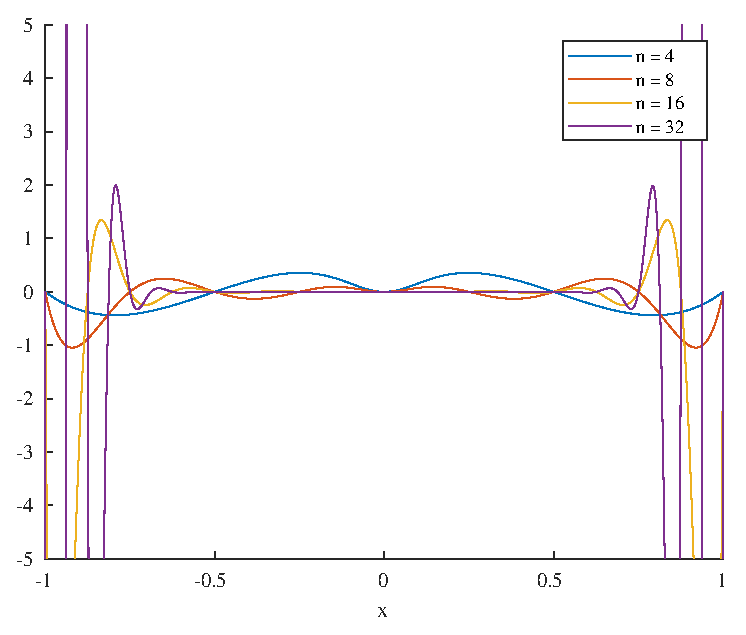
\includegraphics[width=0.8\textwidth]{p7a.eps}
			\caption{Plot of error function $p_n(x) -f(x)$ for polynomial interpolation}
			\label{fig:p7a}
		\end{figure}
		
		\questionpart The script \texttt{p7b.m} was used to generate Table \ref{table:p7b} and Figure \ref{fig:p7b}. The output from the script is in \texttt{p7b\_output.txt}. Based on the table, it seems that $e_n = \bigoh(n^{-4})$ as $n \to \infty$.
		
		\begin{table}[htb!]
			\centering
			\begin{tabular}{@{}rrr@{}}
				\toprule
				$n$ & $e_n$ & Order\\
				\midrule
				4 & \num{2.793e-01} & - \\ 
				8 & \num{5.607e-02} & 2.32 \\
				16 & \num{3.745e-03} & 3.90 \\
				32 & \num{6.546e-04} & 2.52 \\
				64 & \num{4.013e-05} & 4.03\\
				128 & \num{2.521e-06} & 3.99 \\
				\bottomrule
			\end{tabular}
			\caption{$L^\infty$ errors of natural cubic spline interpolation}
			\label{table:p7b}
		\end{table}
		
		\begin{figure}[htb!]
			\centering
			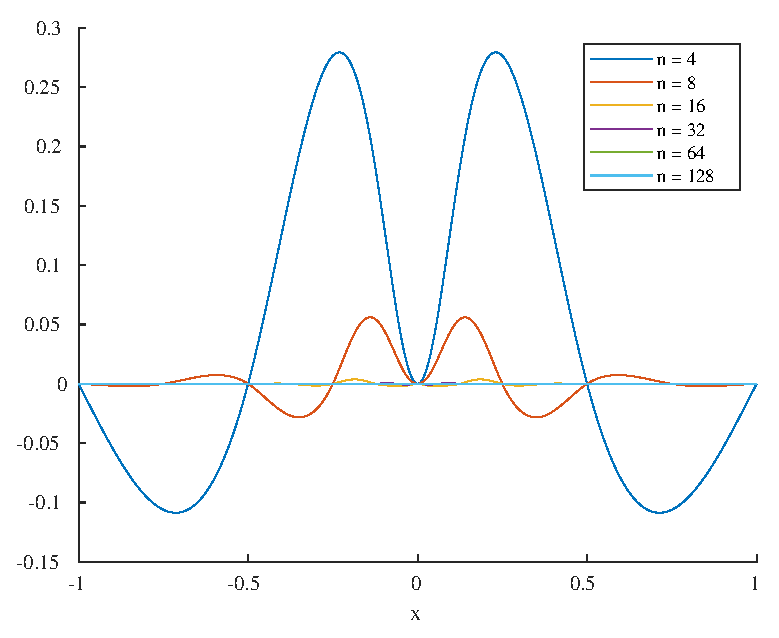
\includegraphics[width=0.8\textwidth]{p7b.eps}
			\caption{Plot of error function $p_n(x) -f(x)$ for natural cubic spline interpolation. Note the smaller scale compared to Figure \ref{fig:p7a}.}
			\label{fig:p7b}
		\end{figure}
	\end{alphaparts}
\end{document}